\section{Simulations \& Subgrid model}
\label{sect:simulationsandsubgrid}

\begin{figure*}
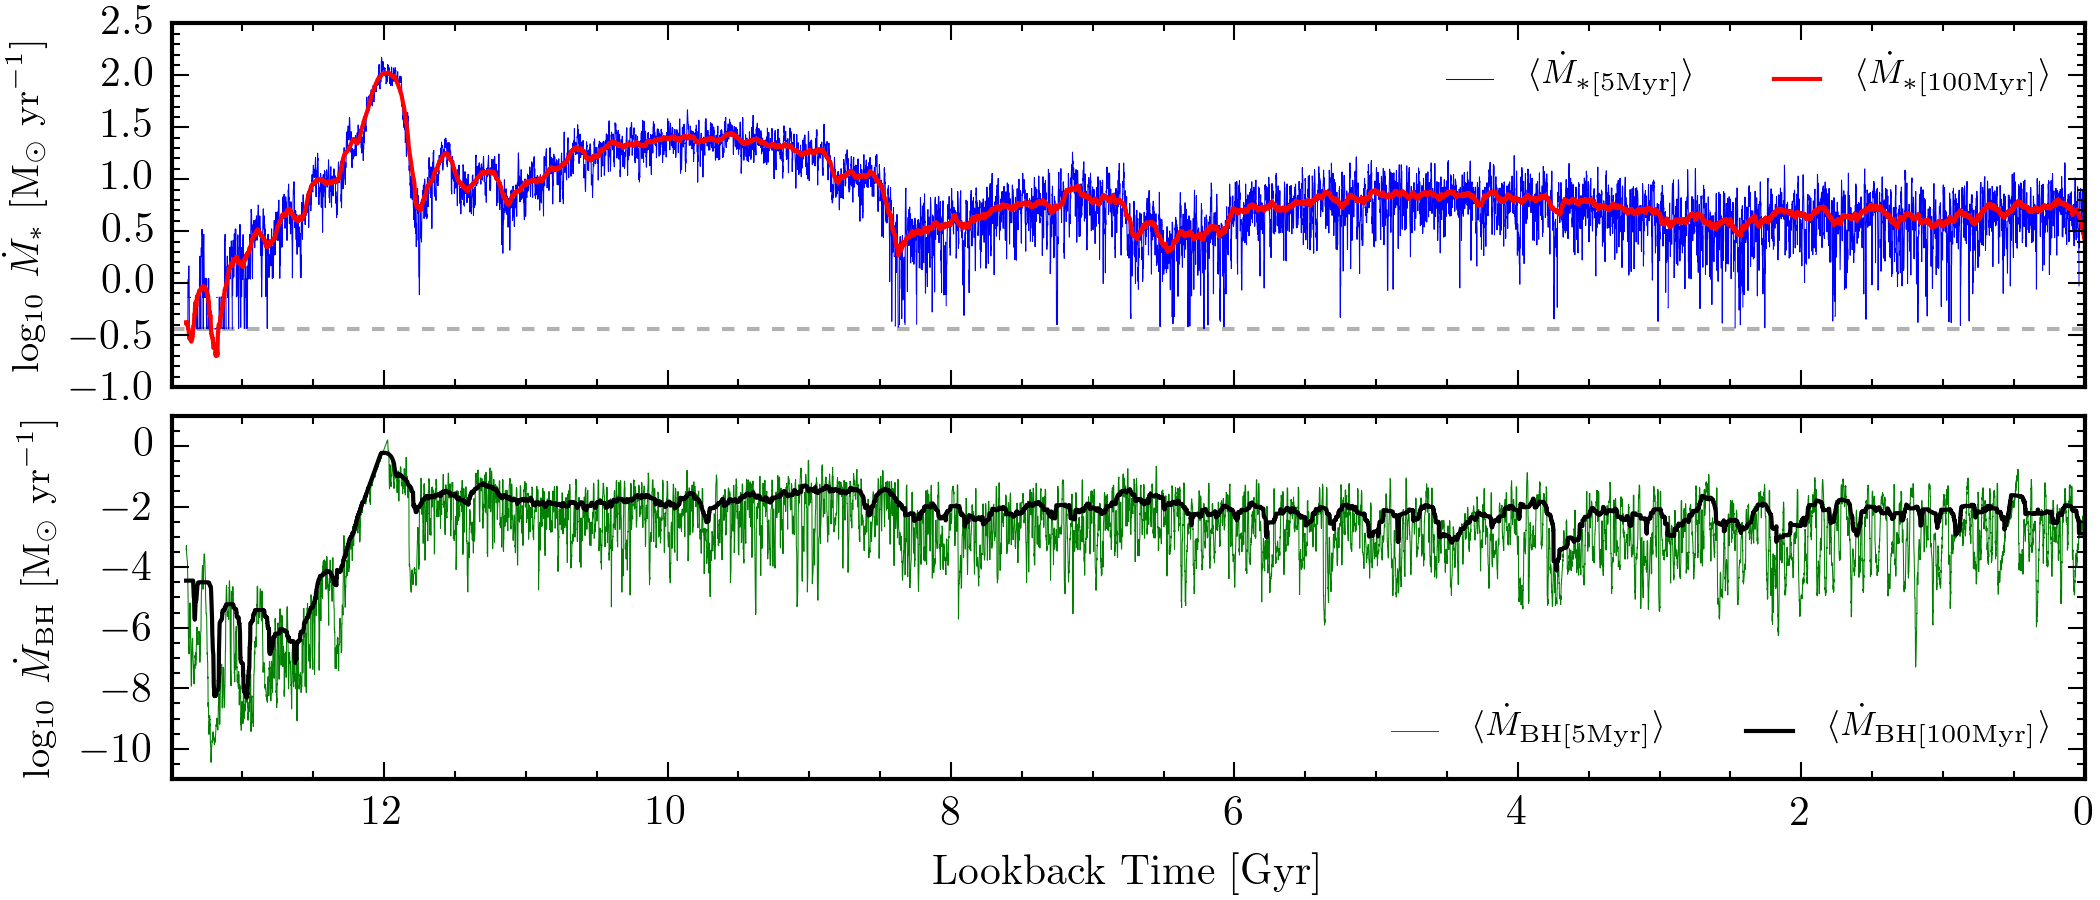
\includegraphics[width=\textwidth]{plots/IndividualHistory}

\caption{Galaxy (top panel) and BH (bottom panel) growth rates as a function of
lookback time for an individual galaxy ({\tt GalaxyID}=20324216,
$M_{\mathrm{200[z=0]}}=10^{13.2}$\Msol, $M_{\mathrm{*[z=0]}}=10^{11.1}$\Msol,
$M_{\mathrm{BH[z=0]}}=10^{8.7}$\Msol). Blue (green) and red (black) lines show
the SFR (BHAR) history averaged over 5~Myr and 100~Myr respectively. When
averaged over short timescales, BHARs can vary by as much as $\approx 4$ dex.
SFRs however vary considerably less over the same time window ($\approx 1$
dex), and generally represent values in much closer agreement to their long
term average rate. In this individual case the long term average trends of SFR
and BHAR yield quite different evolutionary behaviours. As the both the
particle mass and averaging time window is finite, the minimum possible SFR
sampled for a 5~Myr timescale is shown as a dashed grey line.} 

\label{fig:variability}
\end{figure*}

\eagle is a suite of cosmological hydrodynamical simulations comprising a range
of periodic volumes, numerical resolutions and physical models. The simulations
are run using a substantially modified version of the N-body TreePM smoothed
particle hydrodynamics code \gadget-3 \citep{Springel2005}, referred to as
\anarchy \citep[Dalla Vecchia, \textit{in prep}; see also see also appendix A
of][]{Schaye2015}.  For this study we focus on the largest run
(Ref-L0100N1504), a cubic periodic volume of 100 comoving megaparsecs (cMpc) on
each side, containing $1504^{3}$ dark matter particles of mass $9.7 \times
10^{6}$~\Msol and an equal number of baryonic particles with an initial mass of
$1.8 \times 10^{6}$~\Msol. The subgrid parameters are those of the \eagle
reference (\squotes{Ref-}) model, described fully by \citet{Schaye2015}.
Cosmological parameters are those inferred by \citet{Planck2013}, namely:
$\Omega_{\mathrm{m}}=0.307$, $\Omega_{\Lambda}=0.693$,
$\Omega_{\mathrm{b}}=0.04825$, $h = 0.6777$ and $\sigma_{8}=0.8288$.

\subsection{Subgrid model}

Processes operating below the numerical resolution of the simulation are
treated as \squotes{subgrid}, implemented as a series of physical models. A
detailed description of the full subgrid prescription is given by
\citet{Schaye2015}, with consideration to their influence on the reference
model given by \cite{Crain2015}. Here we give only a brief overview:

\begin{itemize}

\item \textit{Radiative cooling and photo-ionisation heating} is implemented as
per \citet{Wiersma2009a}, tracing 11 elements in the presence of the cosmic
microwave background and the evolving, spatially uniform UV/X-ray background of
\citet{HaardtandMadau2001}. 

\item \textit{Star formation} is implemented as a pressure dependent relation
that reproduces the Kennicutt-Schmidt law described by
\citet{Schaye_DallaVecchia2008}. The subsequent \textit{stellar mass loss} via
winds of massive stars and supernovae is computed as per \citet{Wiersma2009b}. 

\item \textit{Stellar feedback} is injected thermally and stochastically
following the method of \citet{DallaVecchia_Schaye2012}.

\item \textit{BH seeding} follows the prescription first introduced by
\citet{Springel2005a}, whereby BHs are introduced as collisionless sink
particles placed in the centres of dark matter haloes more massive than $1.475
\times 10^{10}$\Msol, which do not already contain one. BHs enter the
simulation with a seed mass $m_{\mathrm{seed}} = 1.475 \times 10^{5}$\Msol
and subsequently grow via accretion of surrounding gas or mergers with other
BHs.

\item \textit{BHs grow via accretion} of nearby material at a rate estimated
from the modified Bondi-Hoyle formalism introduced in \citet{RosasGuevara2015}.
In short, the model is an extension of the spherically symmetric case of
\citet{Bondi1944} accounting now for the circularisation velocity of the
surrounding gas, capped at the Eddington limit. Contrary to
\citet{RosasGuevara2015}, we do not use an additional boost factor ($\alpha$).

\item \textit{AGN feedback} is implemented as a single mode, where it is
injected thermally and stochastically into the surrounding interstellar medium
as per \citet{Booth_Schaye2009}. Feedback is performed assuming a single
efficiency, independent of halo mass and accretion rate. 

\end{itemize}

As described by \citet{Crain2015}, the subgrid model parameters are calibrated
to reproduce the observed galaxy stellar mass function, galaxy sizes and
normalisation of the \M{BH}--\M{*,bulge} relation at $z \approx 0.1$.

\subsection{Simulation output}

\subsubsection{Halo and galaxy identification}

Outputs are stored as 29 \squotes{snapshots} between redshifts $z=20$ and $z=0$
at which the complete state of every particle is recorded. In addition, 400
data-lite \squotes{snipshots} are produced, with a typical temporal separation
of $\approx$40-60~Myr. Bound structures are identified in post processing.
First, dark matter haloes are identified using the \squotes{Friends of Friends}
(FOF) algorithm with linking length of $b = 0.2$ times the mean interparticle
separation \citep{Davis1985}.  Then, bound substructures (or
\squotes{subhaloes}) within these haloes are identified with the \subfind
program \citep{Springel2001,Dolag2009} applied to the full particle
distribution (dark matter, gas, stars and BHs). We associate the baryonic
component of each subhalo with a galaxy, defined to be the \textit{central}
galaxy if it hosts the particle with the minimum gravitational potential and
the remainder being classified as \textit{satellites}.

Halo mass, \M{200}, is defined as the total mass enclosed within
$r_{\mathrm{200}}$, the radius at which the mean enclosed density is 200 times
the critical density of the Universe. Galaxy mass, \M{*}, is defined at the
total stellar content belonging to a subhalo within a 30~pkpc spherical
aperture as per \citet{Schaye2015}. 

\subsubsection{Constructing histories of individual galaxies}
\label{sect:individual_galaxies}

In order to accurately trace the evolution of individual galaxies and their
central BH for the analysis in \cref{sect:to_halo}, we require histories of a
higher temporal resolution than is provided by the snipshot output. To do this,
we follow galaxies and their central BH through cosmic time. As a galaxy
descendant may have multiple progenitors, we trace the progenitor galaxy that
is hosted along the \squotes{main progenitor branch} of the merger tree as
defined by \citet{Qu2017}, the branch containing the greatest total mass along
its history.  

BHARs are recorded at each timestep with a typical spacing of $\sim 10^{3} -
10^{4}$~yr, yielding an \squotes{instantaneous} rate. These can then be
time-averaged over longer durations. Quoted \squotes{instantaneous} SFRs are
taken from the snapshot output, where they are computed based on the current
star forming state of the gas contained within the galaxy. Time-averaged SFR
histories are constructed from the stellar particles born within the main
progenitor that reside in the galaxy at the present day. As these particles
store both their birth time and initial mass, collectively they create a robust
history of star formation for that galaxy.  However, as these histories are
sensitive in their resolution to the number of particles sampled, only galaxies
containing more than 200 particles (\M{*[z=0]} $\approx 10^{8.5}$\Msol) are
considered for this study. 

\cref{fig:variability} shows an example history of an individual galaxy's SFR
(top panel) and accretion rate of the central BH (bottom panel) through cosmic
time taken from the methods described above. We show each growth rate
time-averaged over 5~Myr (blue and green lines) and 100~Myr (red and black
lines) to highlight the large difference in variability scatter between the two
timescales. This is particularly severe for BHAR, where values recorded over
short timescales do not return a good approximation of the long term average
rate, differing in value by as much as 4~dex. We have adopted 100~Myr as our
long averaging duration as it reflects an estimate of the effective timescale
for empirical indicators of star formation using the far-infrared \citep[FIR,
the tracer of star formation for the observational studies compared to in
\cref{sect:observations}, see the discussions
by][]{Neistein2014,Volonteri2015a}. Although there are similar features between
SFR and BHAR through time for this individual case (for example a common peak
at a lookback time of 12 Gyr), globally the two histories are quite different. 

\subsection{The \M{BH}--\M{200} relation}
\label{sect:eagle_bhs}

\begin{figure}
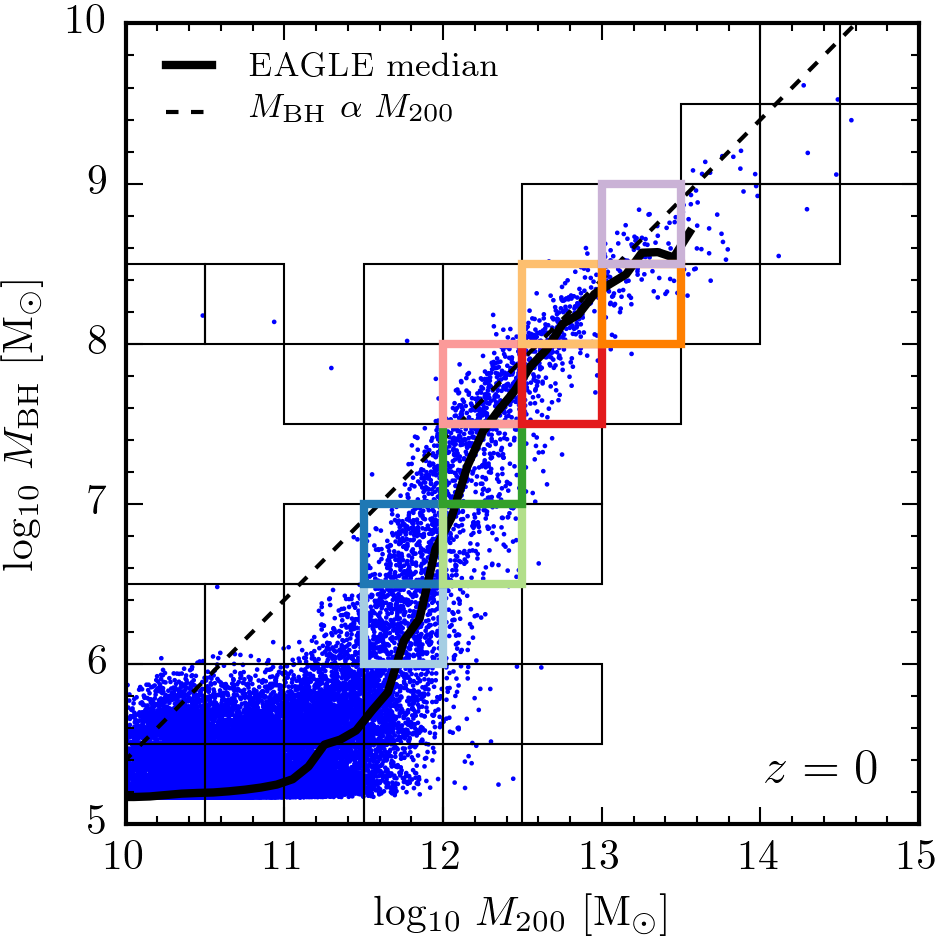
\includegraphics[width=\columnwidth]{plots/BHMvsHM}

\caption{\M{BH}--\M{200} relation for central galaxies at $z=0$, where \M{200}
is the halo mass. Each galaxy is represented by individual blue points and the
median trend is shown as a solid black line. The black dashed line shows a
linear relationship, \M{BH} $\propto$ \M{200}, for reference.  Overlaid
two-dimensional bins are 0.5~dex on each side and contain at least one galaxy.
Nine of these cells are used for the continued investigation in
\cref{sect:discussion} and are outlined in colours that relate to the histories
shown in \cref{fig:avHistory_vs_hm,fig:sfr_vs_bhar_av}.}

\label{fig:bhm_vs_hm}
\end{figure}

\cref{fig:bhm_vs_hm} shows the \M{BH}--\M{200} relation for central galaxies at
$z=0$.  We have plotted \M{BH} as a function of halo mass rather than bulge or
total stellar mass due to the crucial connection that \M{200} has with both SFR
and BHAR (see \cref{sect:to_halo} onwards). We note that the \M{BH}--\M{*}
relation also follows the same behaviour \citep[see Figure 1 of][]{Barber2016}
and throughout this description \M{200} and \M{*} can be interchanged. The
overlaid two dimensional bins are for the continued investigation in
\cref{sect:to_halo}, where they are fully described.  

The empirical relationship between BH mass and that of the classical bulge is
well described by a single power law at high mass \citep[e.g,][with gradient
values of $\alpha \approx 1-1.3$ satisfying
\cref{eq:slope1}]{Magorrian1998,Kormendy2013,McConnellandMa2013}.  Indeed, one
of the calibration parameters of the simulation is to match the normalisation
of this relationship.  However, whereas traditionally this trend has been
linearly extrapolated to lower-mass systems, \eagle predicts a steepening of
the trend.  As a consequence, the relation between BH mass and the mass of the
host galaxy or halo is not well described by a single power law. Interestingly,
a steeper slope at intermediate masses is supported by recent observations of
bulge (or pseudobulge) systems \citep[e.g,][]{Scott2013,Greene2016}.  When
total stellar mass is considered as the independent variable,
\citet{Reines2015} predict Seyfert-like systems yield and alternate
\M{BH}--\M{*} relationship to previously measured early-type systems. However,
each trend is consistent with a linear relation, with Seyfert-like systems
harbouring a lower normalisation.

For \eagle, BHs in massive systems (\M{200} $\gtrsim 10^{12.5}$\Msol) follow an
approximately linear trend with halo mass (compare to the black dashed black
line in \cref{fig:bhm_vs_hm}), but those hosted by haloes with mass \M{200}
$\lesssim 10^{12.5}$\Msol follow a much steeper relation and those in the
lowest mass systems (\M{200} $\lesssim 10^{11.5}$\Msol) plateau at the seed BH
mass.

\citet{Bower2017} argue that multiple physical processes drive the
relation between \M{BH} and \M{200}. In low (high) mass systems stellar (AGN)
feedback regulates the baryonic inflow to the galaxy, suppressing BH (continued
stellar) growth.  There is a critical transition halo mass (\M{200} $\sim
10^{12}$\Msol, hereafter \M{crit}) separating these two regulatory regimes.
Within \M{crit} haloes, neither feedback process is dominant, and as a result
BHs grow at a highly non-linear rate. These phases create the flat,
supra-linear and $\sim$linear regimes of BH growth seen in the integrated
quantities of \cref{fig:bhm_vs_hm} and have important consequences for the
galaxy and BH growth rates investigated throughout this study.

\subsection{Absolute calibration of SFRs}
\label{sect:sfr_calibration}

When comparing to the observed cosmic SFR density, \citet{Furlong2015a} found an
almost constant -0.2~dex offset for redshifts $z \leq 3$.  There is however
continued uncertainty as to the absolute calibration of SFR indicators on which
these observations rely.  For example, \citet{Chang2015} find upon revisiting
this calibration with the addition of WISE photometry to the full SDSS
spectroscopic galaxy sample that the SFRs of local galaxies along the
main-sequence are systematically lower than previously estimated by $\approx
0.2$~dex, yielding good agreement with the \eagle prediction \citep[see Figure
5 of][]{Schaller2015b}.

As the observational datasets compared to in \cref{sect:observations} utilise
an earlier calibration, we \textit{reduce} all observed SFRs by 0.2~dex. The
magnitude of this recalibration is shown as a red arrow in
\cref{fig:stanley2015,fig:delvecchio2015}. This serves to remove the known
global systematic offset, making it simpler to focus on the trends with BHAR
that are the topic of this paper. 
